\documentclass[12pt]{article}

\usepackage{geometry} %for defining page layout
\geometry{total = {8.5in,11in}, margin=1in}

\usepackage{graphicx}
\graphicspath{ {./images/} }

\usepackage{mathtools} %for aligning proof in classwork

\title{QBS 103: Intro to \LaTeX}
\author{Meghan Muse}
\date{August 15, 2024}

\begin{document}

\maketitle % adds additional title

\tableofcontents

\newpage
\section{Typesetting Equations}

Here, we will talk about how to typeset equations.

\subsection{My First Equation}

My equation is $a + b = c$. I can also type it on its own line like this: \[a + b = c\].

\subsection{Mathematical Symbols}

You can use Greek letters by their name, just make sure that you capitalize correctly so that $\delta$ and $\Delta$ are used correctly.

\subsection{Brackets and Parentheses}

Most brackets you can use as normal like this $[x]$ or $(x)$. We can also change the size for nested brackets like this $\bigl( (x) \bigr)$ rather than keeping them all the same size like this $((x))$.

We can also define fractions using brackets as follows: 

\[ \frac{\Delta y}{\Delta x} \]. Notice how everything that is contained within the first curly bracket is in the numerator and everything in the second curly bracket is in the denominator.

\subsection{Integrals, Subscripts, and Superscripts}

Similarly to fractions, everything we want included in a subscript or a superscript is contained in curly brackets. For example, $e^{x}$ or nested like this $x^{a+b^{2}}$. We can do this similarly for subscripts like this: $x_{i}$.

For integrals we use superscript and subscript notation to indicate the bounds like this:  \[ \int\limits_{0}^{1} x^2 \ dx \].Note that the curly brackets are only required for more complex expressions where the entire thing needs to be contained in the superscript or subscript rather than a single number or variable. We can also use a backslash in the middle of the above expression to force a space before the $dx$ unlike how it would otherwise appear: \[ \int\limits_{0}^{1} x^2 dx \]

We use similar formatting for operators such as summation like this:
\[\sum_{i = 1}^{n}\]

\subsection{Conclusions}

In \LaTeX you can write complex equations in plain text and then rely on the compiler to cleanly typeset them for you. These can become as complex as you need but be careful to ensure that the final product looks as you expect it to because it is easy to misplace a bracket that will change how the compiler interprets what you have written.

\newpage
\section{Tables}

I can reference my tables in line like this (Table \ref{tab:SFRP2}).

\begin{table}[h] %h forces it to appear inline at this point.
\begin{tabular}{lccccccc}
\multicolumn{4}{c}{\textbf{Genomic Location}}      & \multicolumn{2}{c}{\textbf{Solid Breast Tissue}} & \multicolumn{2}{c}{\textbf{Breast Milk}} \\
Probe ID   & chr  & pos       & Relation to Island & $\Delta$ M Value               & P Value               & $\Delta$ M Value           & P Value           \\ \hline
cg20881942 & chr4 & 154710826 & Island             & 0.0139                   & 2.51E-05              & 0.0343               & 3.69E-03          \\
cg23910835 & chr4 & 154710900 & N Shore            & 0.017                    & 1.41E-04              & 0.0478               & 1.04E-03          \\
cg07999845 & chr4 & 154710961 & N Shore            & 0.0167                   & 1.45E-06              & 0.0404               & 6.87E-03          \\
cg14435644 & chr4 & 154711070 & N Shore            & 0.0199                   & 1.86E-07              & 0.0734               & 1.28E-05          \\
cg09788843 & chr4 & 154711081 & N Shore            & 0.0128                   & 1.52E-06              & 0.0412               & 2.94E-03          \\
cg24241928 & chr4 & 154711099 & N Shore            & 0.01                     & 8.17E-06              & 0.0291               & 5.76E-04          \\
cg23502475 & chr4 & 154711115 & N Shore            & 0.0092                   & 1.99E-07              & 0.0264               & 5.74E-04          \\
cg13357229 & chr4 & 154711171 & N Shore            & 0.0092                   & 3.44E-05              & 0.0333               & 3.59E-03          \\
cg20727217 & chr4 & 154711280 & N Shore            & 0.0061                   & 3.20E-04              & 0.0158               & 7.31E-03          \\
cg01821854 & chr4 & 154711347 & N Shore            & 0.0064                   & 1.36E-04              & 0.0204               & 1.67E-03         
\end{tabular}
\caption{Age association with DNA methylation of the 10 overlapping hypermethylated probes in solid breast tissue and breast milk that map to the TSS1500 region of \textit{SFRP2}.}
\label{tab:SFRP2}
\end{table}

\section{Formatting}
\subsection{Changing Font Size}
You can change the relative size of text using functions to make some words \tiny{} tiny \normalsize{} and other words \huge{} huge \normalsize{}.


\section{Adding References}

I can cite the article our data came from for the final project like this \cite{Overmyer2021}.

\newpage
\section{In Class Activity}

We can add in and reference figures like this (Figure \ref{fig:Prob}).

\begin{figure}[h]
    \centering
    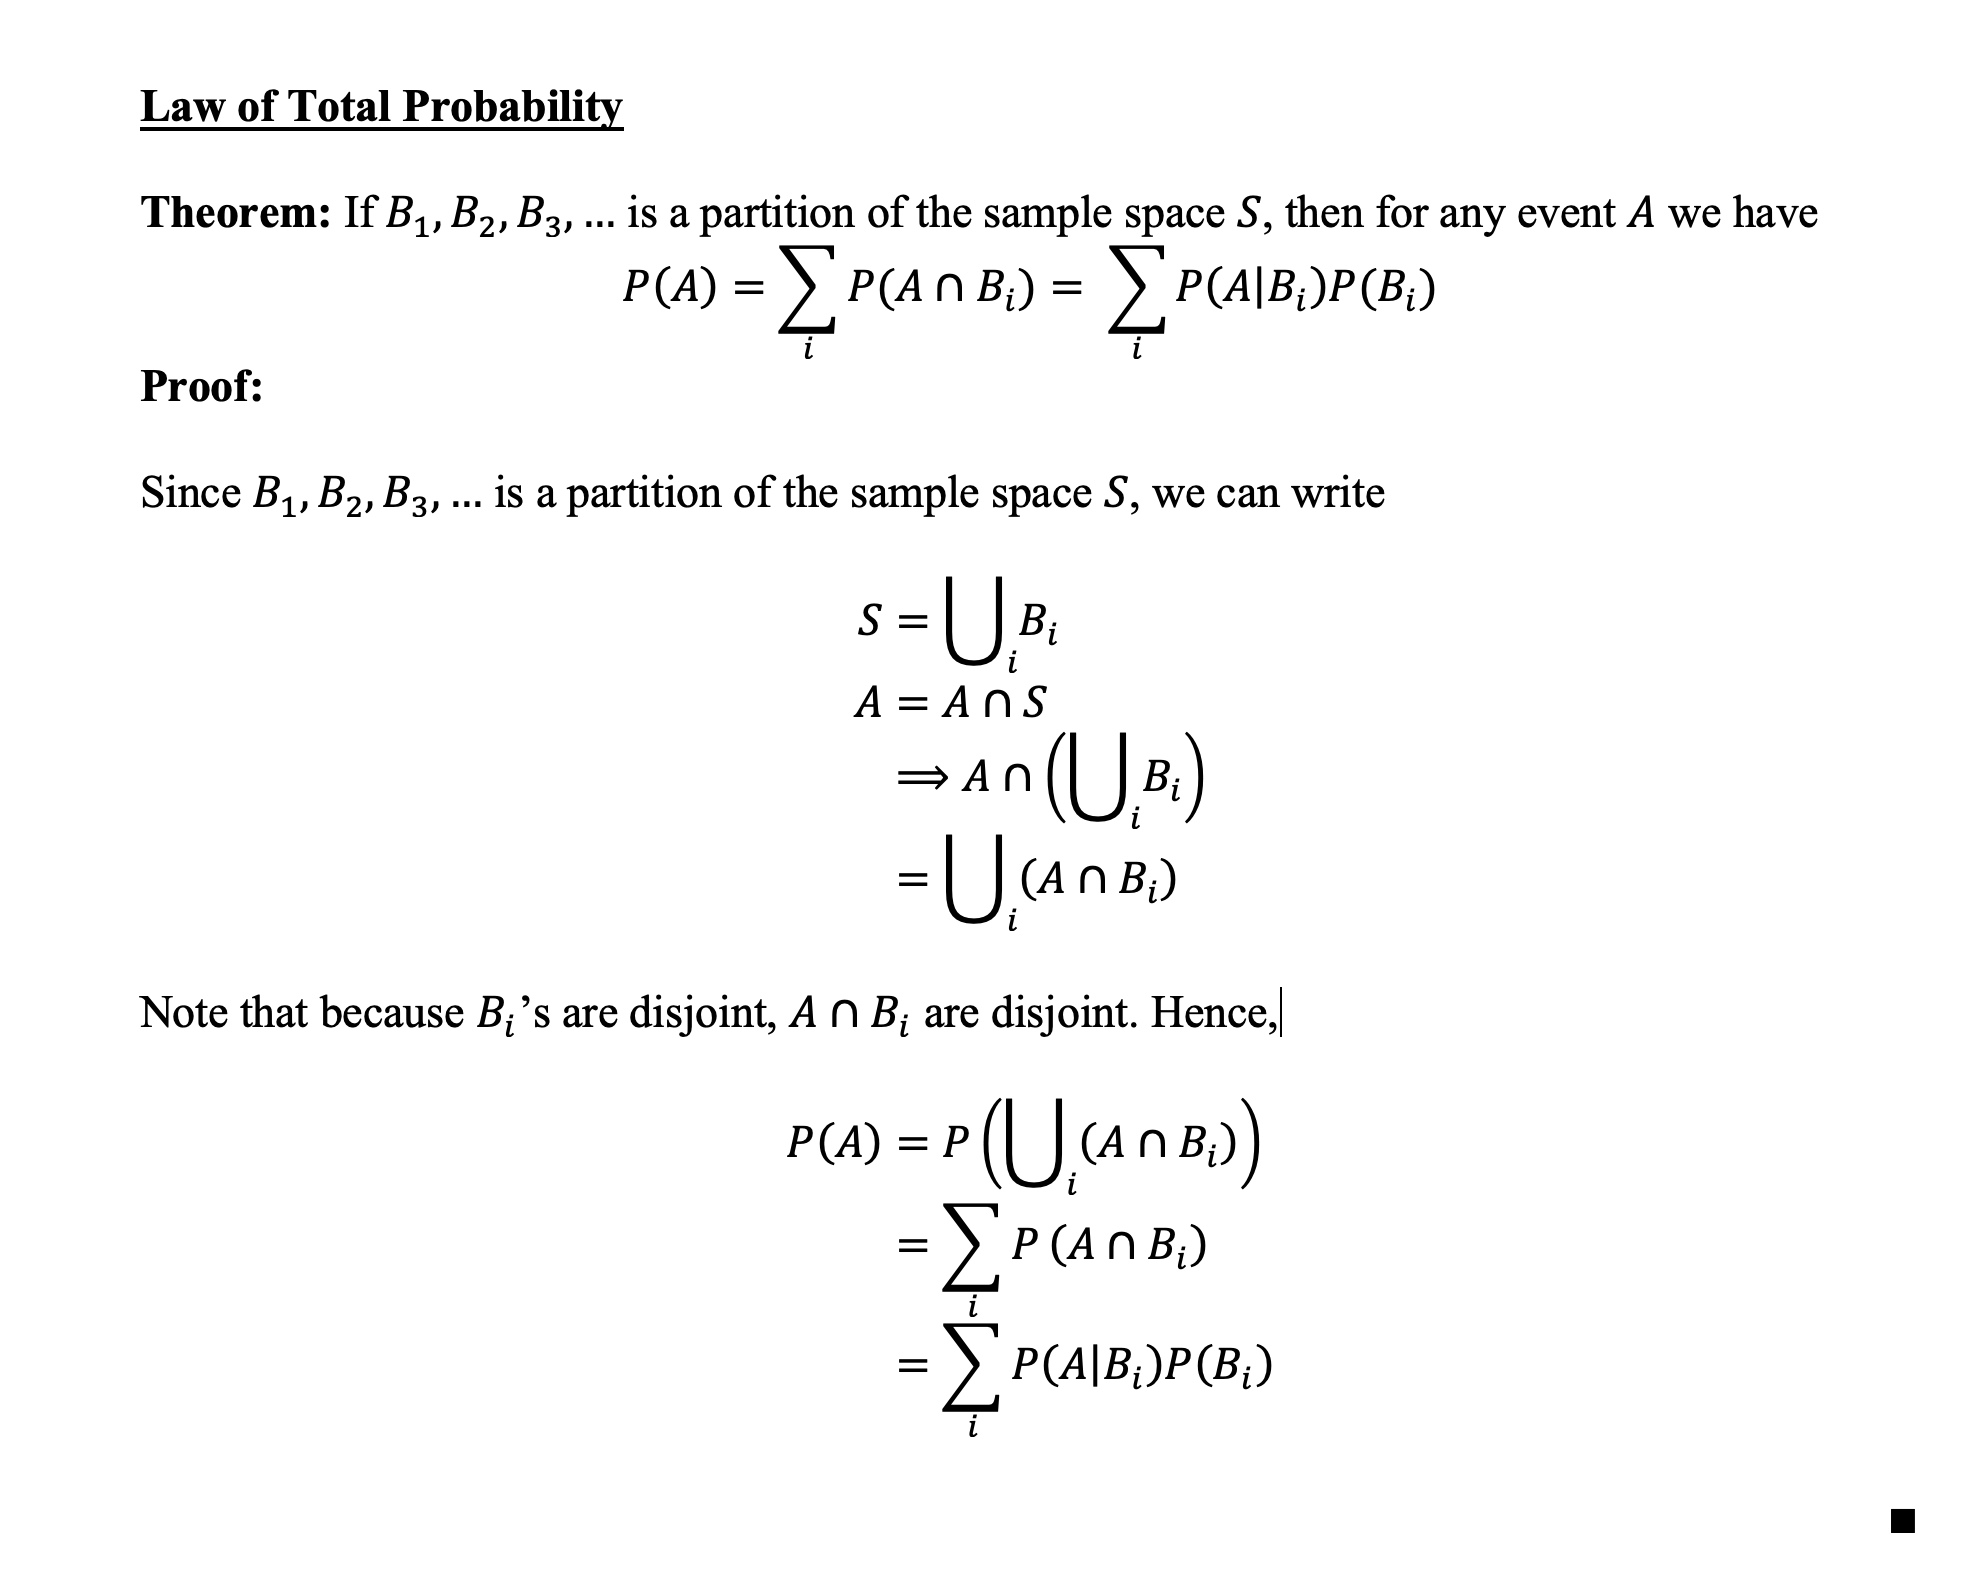
\includegraphics[width = \textwidth]{TotalLawProbability.png}
    \caption{This is the proof for the total law of probability.}
    \label{fig:Prob}
\end{figure}

%\include{LawOfTotalProbability}

\bibliographystyle{pnas2009}
\bibliography{QBS103_refs}

\end{document}
